\documentclass[12pt,preprint]{aastex}
\usepackage[margin=1in]{geometry}
\usepackage{float,amsmath}
%\usepackage{titlesec} %used to format titles
\usepackage{graphicx} %for handling figures
%\usepackage[none]{hyphenat} %disallows hyphenated words
\citestyle{aa}

\begin{document}

\title{HERA Dish Reflectometry} 
\author{Nipanjana Patra, Zaki Ali, Carina Cheng, Dave DeBoer, Gilbert Hsyu, Tsz Kuk Leung, Aaron Parsons}
\maketitle

\section{Introduction}

There are several different sources of instrumental chromaticity for radio
telescope systems that can result in non-ideal performances and unwanted
systematic effects in measured data. One such source is the mismatch between
the impedance of free space and the feed and transmission line, which
results in a partial coupling of the sky signal into the feed while the rest
is reflected back into the space. For any reflector telescope, such as HERA, this signal illuminates the dish and part of it reflects
back and forth several times in between the dish feed and the vertex of the
dish.  Such reflections generate multiple reduced strength copies of the
incident sky signal at various delays, and this produces spurious correlations
in the visibilities of interferometric data. 

To first order, the design specification of HERA elements requires that any
delayed signal, arriving at the feed after a multipath propagation, should be
at the level of $-60dB$ at a delay of $60ns$ relative to the first incident
signal at the feed \citep{parsons_deboer_memo}. This specification was
approximated based on the power level of the cosmological signal in relation to
foreground signals, which is estimated to be six orders of magnitude fainter
\citep{santos_et_al2005,ali_et_al2008,deoliveira2008,jelic_et_al2008,bernardi_et_al2009,bernardi_et_al2010,ghosh_et_al2011}.
Additionally, the $14m$ HERA baselines set a foreground containing
horizon-limit (the wedge) that, with some buffer, sets a delay specification of
$60ns$
\citep{parsons_et_al2012b,vedantham_et_al2012,nithya_et_al2013,liu_et_al2014a,liu_et_al2014b}.

We carry out reflectometry measurements at the HERA element prototype in Green
Bank, WV in order to understand the nature of feed reflections in the dish
and characterize its performance. As HERA progresses as an experiment, it is
necessary to build optimal dishes that aim to minimize the challenges of
chromaticity in our quest for the Epoch of Reionization.

\section{Theory}{\label{sec:theory}}
\begin{figure}[ht!]
\centering
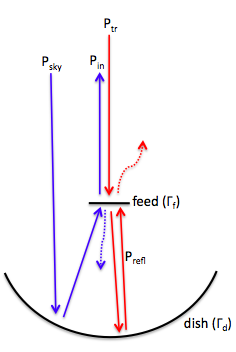
\includegraphics[totalheight=0.3\textheight]{plots/reflection_cartoon.png}
\caption{The blue solid lines represent an original sky signal entering the
feed. A small percentage of it (dashed blue) is reflected off the dish, and it
is these reflections that we are concerned about. In our measurements however,
the reflections measured contain most of the original pulse signal (solid red),
so it is crucial to adjust for this difference in our analysis.}
\label{fig:cartoon}
\end{figure}
Plane waves incident on a parabolic dish
are focussed at the feed with focal height $l$. For a well-designed feed, one
that closely matches the impedance of free space\footnote{The impedance of free space
is $Z_{0} = \mu_{0}c_{0} = \frac{1}{\epsilon_{0}c_{0}} \approx 377\Omega $.},
most of the signal will enter the system while only
a small percentage will be reflected back towards the dish for a secondary
reflection into the feed (blue arrows in Figure \ref{fig:cartoon}). In the
following discussion, we consider a reflection off the feed and the
subsequent reflection off the dish as one reflection.

Quantitatively, if the incident power from the sky signal is $P_{sky}$, the feed
reflection coefficient is $\Gamma_{f}$, and the dish reflection
coefficient is $\Gamma_{d}$, then the net power entering the feed after an
$n^{th}$ reflection off the feed and the dish is:

\begin{equation}\label{eqn:series1}
P_{in} =  P_{sky}(1-\Gamma_{f})[1+ \Gamma_{f}\Gamma_{d} e^{i\phi}+ (\Gamma_{f}\Gamma_{d})^2e^{i2\phi}+ ....+ (\Gamma_{f}\Gamma_{d})^{n}e^{in\phi}]
\end{equation}

where, $\phi = 2l({2\pi \over c})f$ is the propagation delay of a lightwave of frequency $f$ due to a reflection over a focal distance $l$. Notable here is, upon first incidence, the sky signal is focussed onto the feed from the entire dish and the dish reflection coefficient $\Gamma_{d}$ is $1$ for the first incidence. Back and forth reflection of the signal in between the feed and the dish, however, occurs from only a part of the dish which is shadowed by the feed. Therefore, in this case, $\Gamma_{d} < 1$.
Simplifying:
\begin{eqnarray}\label{eqn:ratio1}
{P_{in} \over P_{sky} } & = & (1-\Gamma_{f})[1+ \Gamma_{f}\Gamma_{d} e^{i\phi}+ (\Gamma_{f}\Gamma_{d})^2e^{i2\phi}+ ....+ (\Gamma_{f}\Gamma_{d})^{n}e^{in\phi}] \nonumber\\
      & = & (1-\Gamma_{f}) \displaystyle\sum\limits_{n=0}^{n} [\Gamma_{f}\Gamma_{d}e^{i \phi}]^{n}\nonumber\\
      & = & (1-\Gamma_{f})+(1-\Gamma_{f}) \displaystyle\sum\limits_{n=1}^{n} [\Gamma_{f}\Gamma_{d}e^{i \phi}]^{n}
\end{eqnarray}

The ratio in Equation \ref{eqn:ratio1} quantifies the amount of power received
w ith respect to the incident sky power. Realistically, the incident sky power
is not easily quantifiable, but it is a quantity we need to know to accurately
characterize reflections.  
%The right hand side of this equation consists of system parameters which are all chromatic i.e, functions of frequency.  


%Reflections cause the sky signal to appear at various delays. We aim to measure
%the relative signal strength at those various delays, referred to as the
%``delay spectrum" hereafter, to estimate levels of reflections in between the
%feed and the dish apex.
 
%We employ the reciprocity theorem for antennas in our experimental set-up.
%More specifically, our experimental set-up differs from measuring sky signal
%reflections since we send a pulse that is to be transmitted from the feed
%before receiving it again. This results in a reversed situation - most of our
%original signal is transmitted from the feed to be reflected from the dish,
%while a small percentage reflects back down the cable (red arrows in Figure
%\ref{fig:cartoon}). Therefore, since our measurement is carried out in
%transmitting mode while an observation would be carried out in receiving mode,
%we correct our results in order to map them to represent real observations.

In our experimental set-up, instead of using sky signal, we employ
our feed as a transmitter and transmit a pulse. If the initial pulse is a broadband signal,
$P_{tr}$, sent to the feed antenna via a $75m$ long cable by a vector network
analyser (VNA), a delay domain measurement of the system is accomplished by
taking the Fourier transform of the measured complex return loss of the feed. When the signal is incident on
the feed, part of the incident power ($\Gamma_{f}$) is reflected back to the
measuring device (dashed red arrows in Figure \ref{fig:cartoon}) and
$(1-\Gamma_{f})$ is radiated by the feed (solid red arrows in Figure
\ref{fig:cartoon}) which illuminates the dish. While most of the incident signal is reflected back into the space by the dish, the reflected signal from the dish vertex returns to
the feed. This incident signal is now
reflected back and forth in between the feed and the dish much like the sky
signal reflection discussed previously.  Hence, if $P_{r}$ is the power
incident back on the feed for the first time then the reflected power $P_{ref}$
back into the VNA would be:

\begin{equation}\label{eqn:series2}
P_{ref} =  P_{r}(1-\Gamma_{f})[1+ \Gamma_{f}\Gamma_{d} e^{i\phi}+ (\Gamma_{f}\Gamma_{d})^2e^{i2\phi}+ ....+ (\Gamma_{f}\Gamma_{d})^{n}e^{in\phi}]
\end{equation}
 
Once again, note that we consider one reflection from the feed and its subsequent reflection from the dish as one reflection in total. Equation \ref{eqn:series2} is similar to Equation \ref{eqn:series1}, with different incident powers.

Recall that $P_{r}$ is the initial power that is incident back on the feed, which is just the feed radiated power reflected off the dish:
 
\begin{equation}
P_{r}= \Gamma_{d}(1-\Gamma_f)e^{i\phi} P_{tr}
\end{equation}

Also note that the first reflection of the signal sent by the VNA occurs at the antenna end. Hence the total returned power $P_{ret}$, to the VNA  would be:

\begin{eqnarray}
P_{ret} & = & \Gamma_{f}P_{tr} \nonumber\\ 
 & + &   \Gamma_{d}(1-\Gamma_f)e^{i\phi} P_{tr}(1-\Gamma_{f}) [1+ \Gamma_{f}\Gamma_{d} e^{i\phi}+  ....+ (\Gamma_{f}\Gamma_{d})^{n}e^{in\phi}]\nonumber\\
 \end{eqnarray}
 
Simplifying:
 
  \begin{eqnarray}\label{eqn:ratio2}
 {P_{ret} \over P_{tr} } & = & \Gamma_{f}
  +  \Gamma_{d}(1-\Gamma_f)^{2} [e^{i\phi}+ \Gamma_{f}\Gamma_{d} e^{i2\phi}+  ....+ (\Gamma_{f}\Gamma_{d})^{n}e^{i n\phi}]\nonumber\\
  & = & \Gamma_{f} + { (1-\Gamma_f)^{2}\over \Gamma_{f} } \displaystyle\sum\limits_{n=1}^{n} [\Gamma_{f}\Gamma_{d}e^{i\phi}]^{n}
   \nonumber\\
\end{eqnarray}

The ratio in Equation \ref{eqn:ratio2} is the returned power to the VNA with
respect to the transmitted power sent by the VNA. It is identical to the sky
observation case in Equation \ref{eqn:ratio1} but differs by two factors. The
first factor corresponds to an additive amplitude difference arising from
$\Gamma_{f}$, which physically accounts for the initial reflection at the feed.
The second difference is a multiplicative term which informs us about the first
reflection. Both of these terms need to be corrected for in order to relate our
measurements to real observations.
%Therefore, because our measurement is carried out in transmitting mode
%while a sky observation would be carried out in receiving mode, we correct our
%results in order to map them real observations.

The VNA measures the magnitude and phase of the quantity ${P_{ret}\over P_{tr}}$
as a function of frequency as shown in Figure \ref{fig:freq}. In our measurement
set-up, the first reflection occurs at the antenna terminal $\Gamma_{f}$, so
$({P_{ret} \over P_{tr} }  - \Gamma_{f}) $ gives an estimate of the delay
spectrum of the sky signal. In delay domain, the relative signal strength at
zero delay represents the factor $\Gamma_{f}$ while the signal strength at any
other delay represents any delayed signal that enters the feed after being
reflected from the feed surroundings. 

\section{Methodology}{\label{sec:methods}}

Our reflectometry measurements are made using a prototype HERA dish (Figure
\ref{fig:heradish}) at NRAO in Green Bank, WV. The dish is a $14\,m$ diameter
parabolic reflector structurally supported with 3 telephone poles. The
reflective material is made up of wire mesh that is attached to PVC
pipes, forming the parabolic shape of the dish. With the current iteration of
the HERA dish, the feed consists of a PAPER dipole encased in a cylindrical cage
encompassing the backplane. The PAPER feed and the backplane (which is aimed at
preventing feed-to-feed interaction between neighboring dishes) is raised and
lowered by a three-pulley system. The focal height of the dish is $4.5m$
($\sim{14.76}$ft).  

\begin{figure}[ht!]
\centering
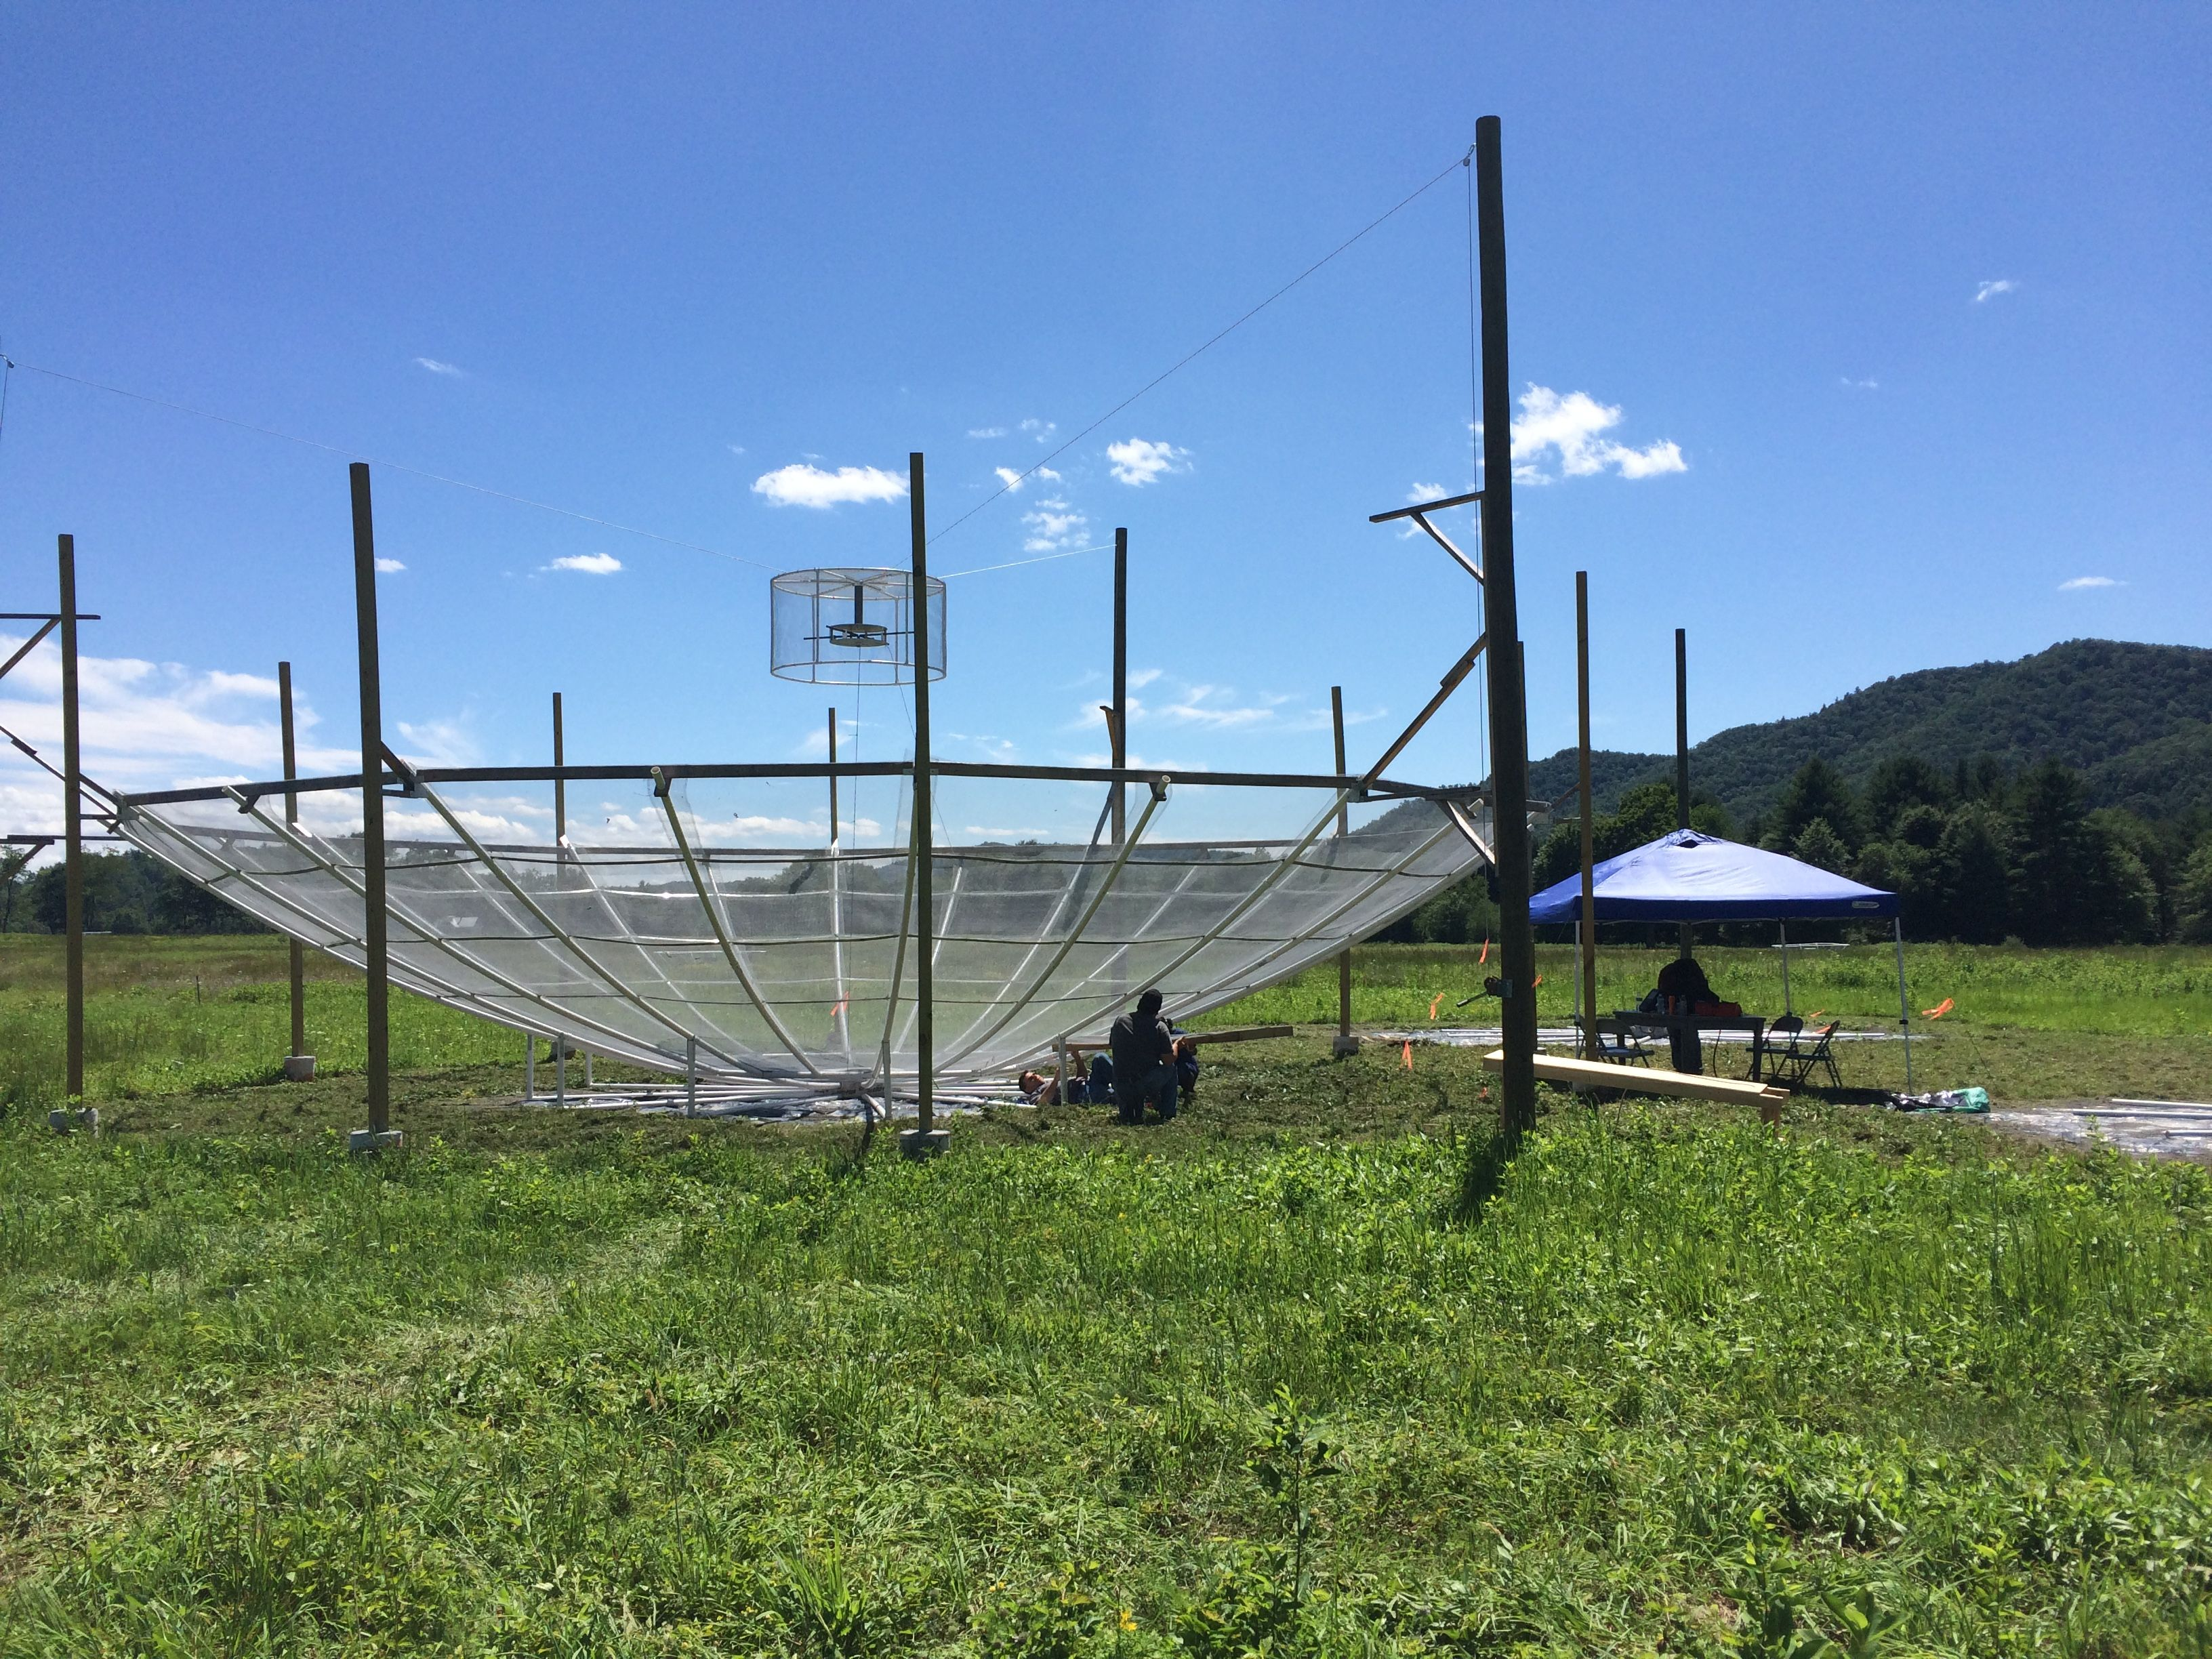
\includegraphics[trim={2cm 20cm 30cm 15cm},clip, totalheight=0.3\textheight]{plots/heradish.jpg}
\caption{HERA dish and feed at the Green Bank NRAO site.}
\label{fig:heradish}
\end{figure}

%The heights measured in our experiment were made from
%the balun to the top of the concrete hub. However, the focal height should be
%measured from the backplane to point where the wire mesh would intersect the
%concrete hub at the vertex of the dish. To account for this height discrepency,
%we add 1.96 ft to all of our measured heights. These are the heights quoted in
%the plots.[XXX not done yet but will be done]
Our measurements are made with a FieldFox in VNA mode. In this mode, a pulse
is generated in the FieldFox and sent through a $75ft$ $50\Omega$ cable that
connects to the feed with a 4:1 passive balun. The magnitude and phase of the complex return loss is measured between 50 to $500MHz$ over 1024 frequency channels which gives frequency resolution of 0.44MHz. Delay resolution of the measurements is $\Delta{t}=2.22ns$.
In addition, we note that the round trip of a reflection from feed to the dish
is $9m$, which corresponds to a delay of $30ns$.


%Feed heights quoted in our measurements represent the distance from the balun to
%the top of the central concrete hub. However, the actual focal height
%of the dish represents the distance from the backplane of the feed to the dish's
%wire mesh, which intersects the concrete hub between the ground and the top of
%the hub. A 
%XXX get discrepancy distance from DaveD. (1.7 ft from the bottom plate of
%sandwich to the top of the the cage and .26 ft from the top of the concrete hub
%to the middle where the parabola starts)

%need to add in third : Antenna feed focal length 4.5 m which corresponds to a
%signal propagation delay of 0.3 ns. Hence, subsequent reflections from the dish
%vertex are expected to be at a delay which is integral multiple of 0.3 nS.
\begin{figure}[ht!]
\centering
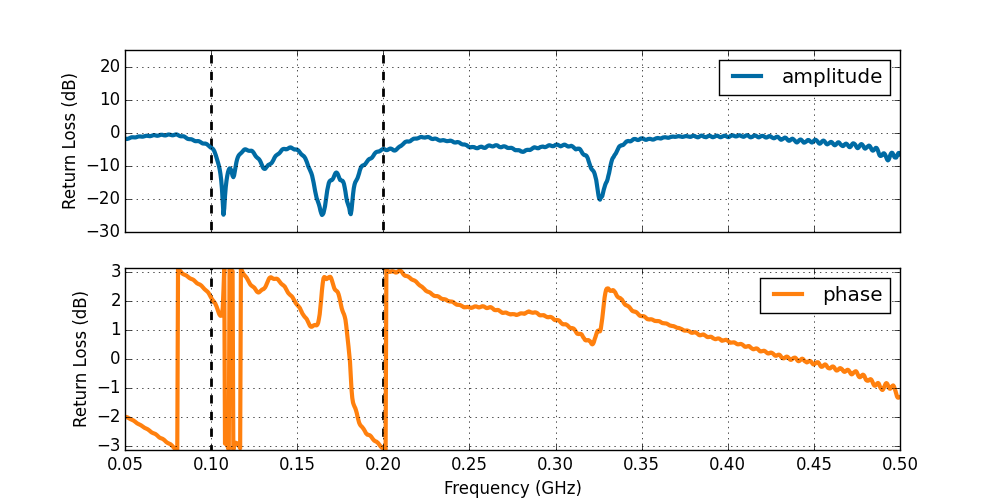
\includegraphics[totalheight=0.4\textheight]{plots/frequency_amp_phase_fullbw.png}
\caption{Amplitude and phase of the measured return loss. Colored dashed lines
mark three different frequency bands: $140-160MHz$, $100-200MHz$, and
$50-250MHz$.}
\label{fig:freq}
\end{figure}

Frequency domain data, as shown in Figure \ref{fig:freq}, can be Fourier-transformed to compute the return loss in the delay domain. Since the measured data is band limited between 50 to 500~MHz which is analogous to multiply the measured data by a square window function, in delay domain, the response is convolved with a $sinc$ function. This may result in excess power at high
delays due to the sidelobes of the $sinc$ function. Hence, appropriate windowing of the measured data set is necessary before taking the Fourier transform.
We have chosen a Hamming window for our analysis. The effectiveness of this
window function compared to others is illustrated in Figure
\ref{fig:window}. 

As mentioned in Section \ref{sec:theory}, there is a mis-match in amplitude
between the reflections that we measure (originating from the FieldFox pulse)
and reflections produced by sky signal. The reflections that we measure (at high
delays) must be lowered by a factor to represent weaker reflections that would
occur after most of the sky signal is received by the feed. For our
compensation, we multiply our entire delay spectrum by its DC component, which is the feed reflection coefficient $\Gamma_{f}$, and also divide by ($1-\Gamma_{f}$). In other words, this correction factor equates Equation \ref{eqn:ratio2} with Equation \ref{eqn:ratio1}. 
We note that this correction is only accurate at high delays where our
reflections of interest occur. At low delays, our spectrum amplitude should be
increased to represent the original sky signal, but we do not apply this
correction because it is not relevant to our analysis.

\begin{figure}[H]
\centering
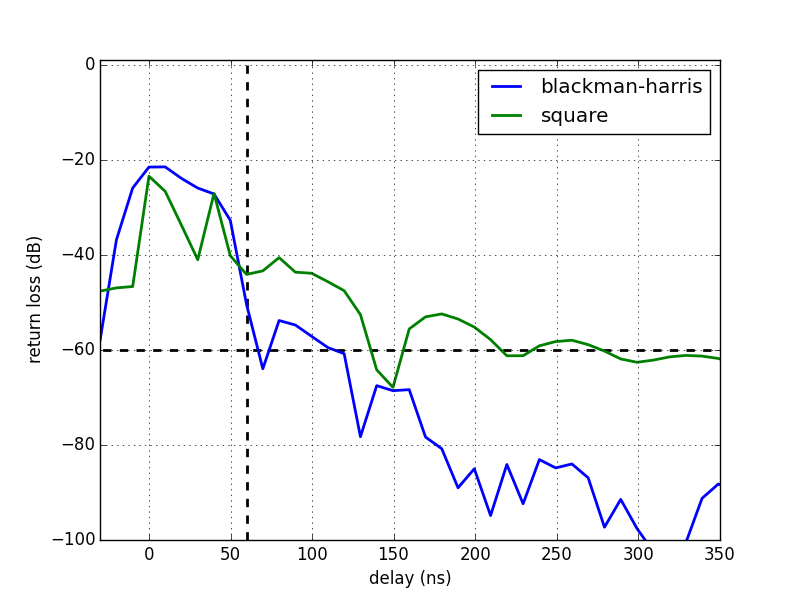
\includegraphics[totalheight=0.4\textheight]{plots/bh_vs_sq.png}
\caption{Delay plot, produced for the PAPER bandwidth ($100MHz-200MHz$) by taking the Fourier transform of the measured return loss using four different window functions: Blackman-Harris, Hamming, Hanning, and square. }
\label{fig:window}
\end{figure}

\section{Results}

Figure \ref{fig:freq} shows the return loss for a frequency bandwidth of $50$ to
$500MHz$. This measurement was taken with the feed suspended at $13.96ft$, which
was our closest measurement to the actual focal height.  Because the return
loss is the ratio of the power received to the power transmitted, higher
reflections can clearly be seen outside of the PAPER bandwidth. This is not
surprising, since the feed is tuned specifically for PAPER. The return loss
minima are locations where our feed is well-matched to free space.

In Figure \ref{fig:3bands}, the return loss we measure is plotted versus delay for three
chosen bandwidths: the HERA bandwidth, the PAPER bandwidth, and a typical power
spectra bandwidth when using a Hamming window function. Two additional measurements, using data taken in 2014 using the first prototype HERA dish in the Berkeley Hills, are also plotted using two different bandwidths. One of the main differences between the Green Bank and Berkeley measurements is that the feed was not encompassed in a cage for the Berkeley data. 

From the plot, we see that the delay response of an antenna is dependent on the band chosen for the Fourier transform.  As one might expect, in regions
where feed return loss is low, reflections are minimized.  Thus, one cannot ignore that these measurements were performed
using a PAPER-style feed tuned for efficient operation over a $100-200MHz$ bandwidth.  Fourier transforms taken over wider bands
become dominated by the feed performance in regions outside the operating band, making the resultant delay profiles less relevant
for the power-spectrum performance of the HERA instrument.  Conversely, when performing transforms over much 
narrow bands (the windowed $20MHz$ bands typical of PAPER analysis), the width of the resulting delay profile
becomes dominated by sidelobes of low-delay emission interacting with the narrow bandwidth kernel.  
Although this may appear to be a relevant performance metric
for PAPER-style power spectrum analysis, such an analysis typically pre-filters out low-delay emission using wide bandwidths precisely to avoid
sidelobes from low-delay emission.  Hence, the most relevant delay-spectrum performance profile is that taken using the $100-200MHz$ band.

\begin{figure}[H]
\centering
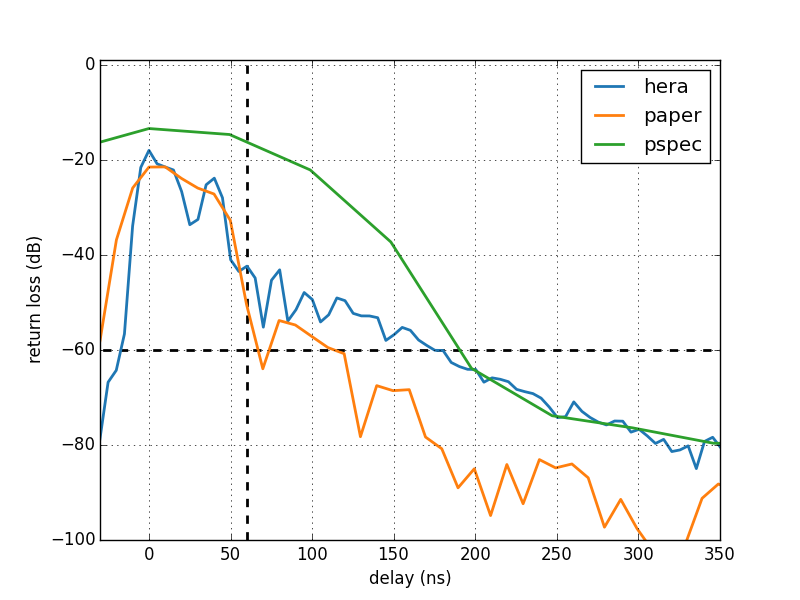
\includegraphics[totalheight=0.4\textheight]{plots/delay3_window.png}
\caption{Delay plots produced using a Hamming window function for 5 different cases. Three of the cases correspond to measurements taken in Green Bank for three frequency bandwidths: $50MHz-250MHz$ (HERA bandwidth), $100MHz-200MHz$ (PAPER bandwidth), $140MHz-160MHz$ (typical power spectrum bandwidth). Two of the cases correspond to measurements taken in 2014 of the first prototype HERA dish in Berkeley (without a feed cage). Of these, we plot data for two frequency bandwidths: $100MHz-200MHz$ (PAPER bandwidth), and $50MHz-1000MHz$ (full bandwidth used by the VNA). For the PAPER bandwidth data, we follow the same Fourier-transform analysis as the others, while the full bandwidth data is produced directly by the VNA. The black dashed lines illustrate our ``60 by 60" specification.}
\label{fig:3bands}
\end{figure} 

In the $100-200MHz$ delay profile, we see a delay response of $-50dB$ at $60ns$, which slopes down to $-60dB$ at $\sim120ns$.  Insofar as
this does not achieve $-60dB$ attenuation at $60ns$, this indicates that the HERA system under test does not meet specification. However, we can learn additional information by evaluating
different feed components. 

\begin{figure}[ht!]
\centering
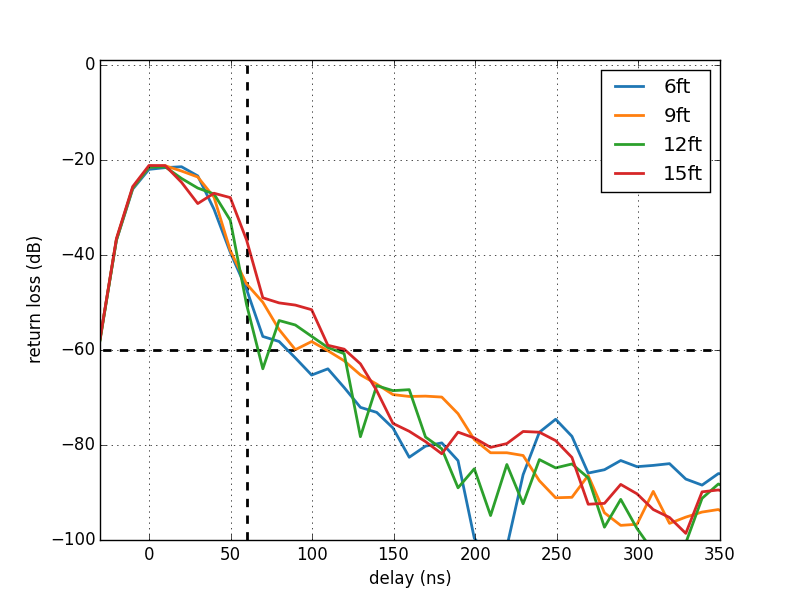
\includegraphics[totalheight=0.4\textheight]{plots/delay_heights_paper.png}
\caption{Delay plots produced using a Hamming window function for 4 different feed heights and the PAPER bandwidth ($100MHz-200MHz$). The black dashed lines illustrate our ``60 by 60" specification.}
\label{fig:elevator}
\end{figure}


Figure \ref{fig:elevator} is again a delay plot of the return loss, but for
four different feed suspension heights. We use the PAPER bandwidth and note
that the measurements are near identical at low delays, implying that low delay
reflections are caused primarily by reflections within the feed cage. However,
at higher delays we notice discrepancies between the different heights.

In addition, Figure \ref{fig:outofthedish} presents measurements taken of the feed
away from the dish. Echosorb is placed under the feed for some of the
measurements, with the expectation that it will prevent any reflections off the
ground. Measurements are also taken of the feed inside its metal cage in
various configurations. It is shown that the feed performs best without the cage and with the absorber. 

From these various measurements, we find that the feed itself is responsible for a significant portion of the structure up to $60ns$ and
that the cylindrical cage may be contributing up to $20ns$ to the width of the delay profile. We note that this depends strongly
on its coupling to structures around it. Structure beyond $60ns$ appears to scale
with the height of the feed above the dish, making reflections off the dish the likely culprit.

\begin{figure}[H]
\centering
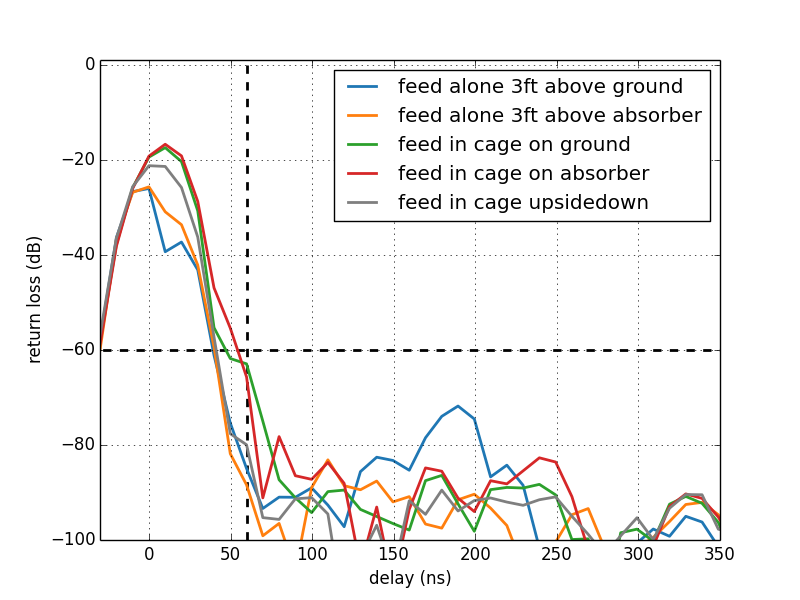
\includegraphics[totalheight=0.4\textheight]{plots/delay_feed.png}
\caption{Delay plots produced using a Hamming window function for different lone feed configurations and the PAPER bandwidth ($100MHz-200MHz$). The black dashed lines illustrate our ``60 by 60" specification.}
\label{fig:outofthedish}
\end{figure}

\section{Conclusion}

The delay-domain performance of the HERA dish is central to HERA's function as a power spectrum instrument.
As we have seen, reflectometry measurements can help characterize HERA's performance in this domain, and
as Equation \ref{eqn:ratio1} shows, these measurements must be adjusted for a difference in transmission/reflection
at the first feed encounter in order to be interpreted as the delay response of an antenna relative to an incident
plane wave from the sky.  We also see that the choice of windowing function is critical for accurately measuring the
antenna delay response at higher delays, where sidelobes from much higher amplitude responses at small delays can easily
dominate.  We find Hamming, Hanning, and Blackman-Harris windows to be generally adequate, but square windowing functions are not.
Given the critical nature of the windowing function, we recommend that all reflectometry measurements be performed in the
frequency domain, so that the data analyst can manually implement the final Fourier transform with the appropriate window.

Taken all together, we summarize that the first version of the HERA dish, with a PAPER-style feed and cylindrical cage, is close to meeting
specification, but will require additional work to fall below $-60dB$ at $60ns$.  Given that the width of the delay response is a convolution
of the feed response and the dish reflections, it is not possible to perfectly decouple the response of the feed from that of the dish.
It may be possible to achieve enough of a reduction to meet specification by modifying the feed.
Given that previous measurements using a PAPER feed with a simple backplane exhibit structure above $-60dB$ at $60ns$,
we deduce that these advances will most likely require improving the feed return loss.  We also recommend re-investigating the scattering
cone for reducing standing waves between the feed and dish.  Finally, given the proximity of our measurements to the rough 
specification that was adopted for 
HERA of $-60dB$ attenuation at $60ns$, we recommend reinvestigating this specification to determine more accurately the impact of 
the element's current delay performance on HERA science.  We suspect that, at the level of $-50dB$ at $60ns$ and $-60dB$ at $120ns$, this
performance may indeed be adequate for the delay-domain power spectrum analysis for which HERA has been optimized.

\bibliographystyle{apj}
\bibliography{biblio}


\end{document}
